\begin{frame}
    \frametitle{Incorporate Real CSZ Bathymetry in Mesh}
    \begin{figure}
        \centering
        \includegraphics[width=0.95\textwidth]{JMM/images/meshes/CSZ-lat-lon-animation.mp4}
        \caption{Animation showing \href{https://www.gebco.net/data_and_products/gridded_bathymetry_data/}{GEBCO} bathymetry data and mesh of a quadrilateral patch of the CSZ using the meshing algorithm described previously}
    \end{figure}
\end{frame}

\begin{frame}
    \frametitle{Incorporate Real CSZ Bathymetry in Mesh}
    \begin{figure}
        \centering
        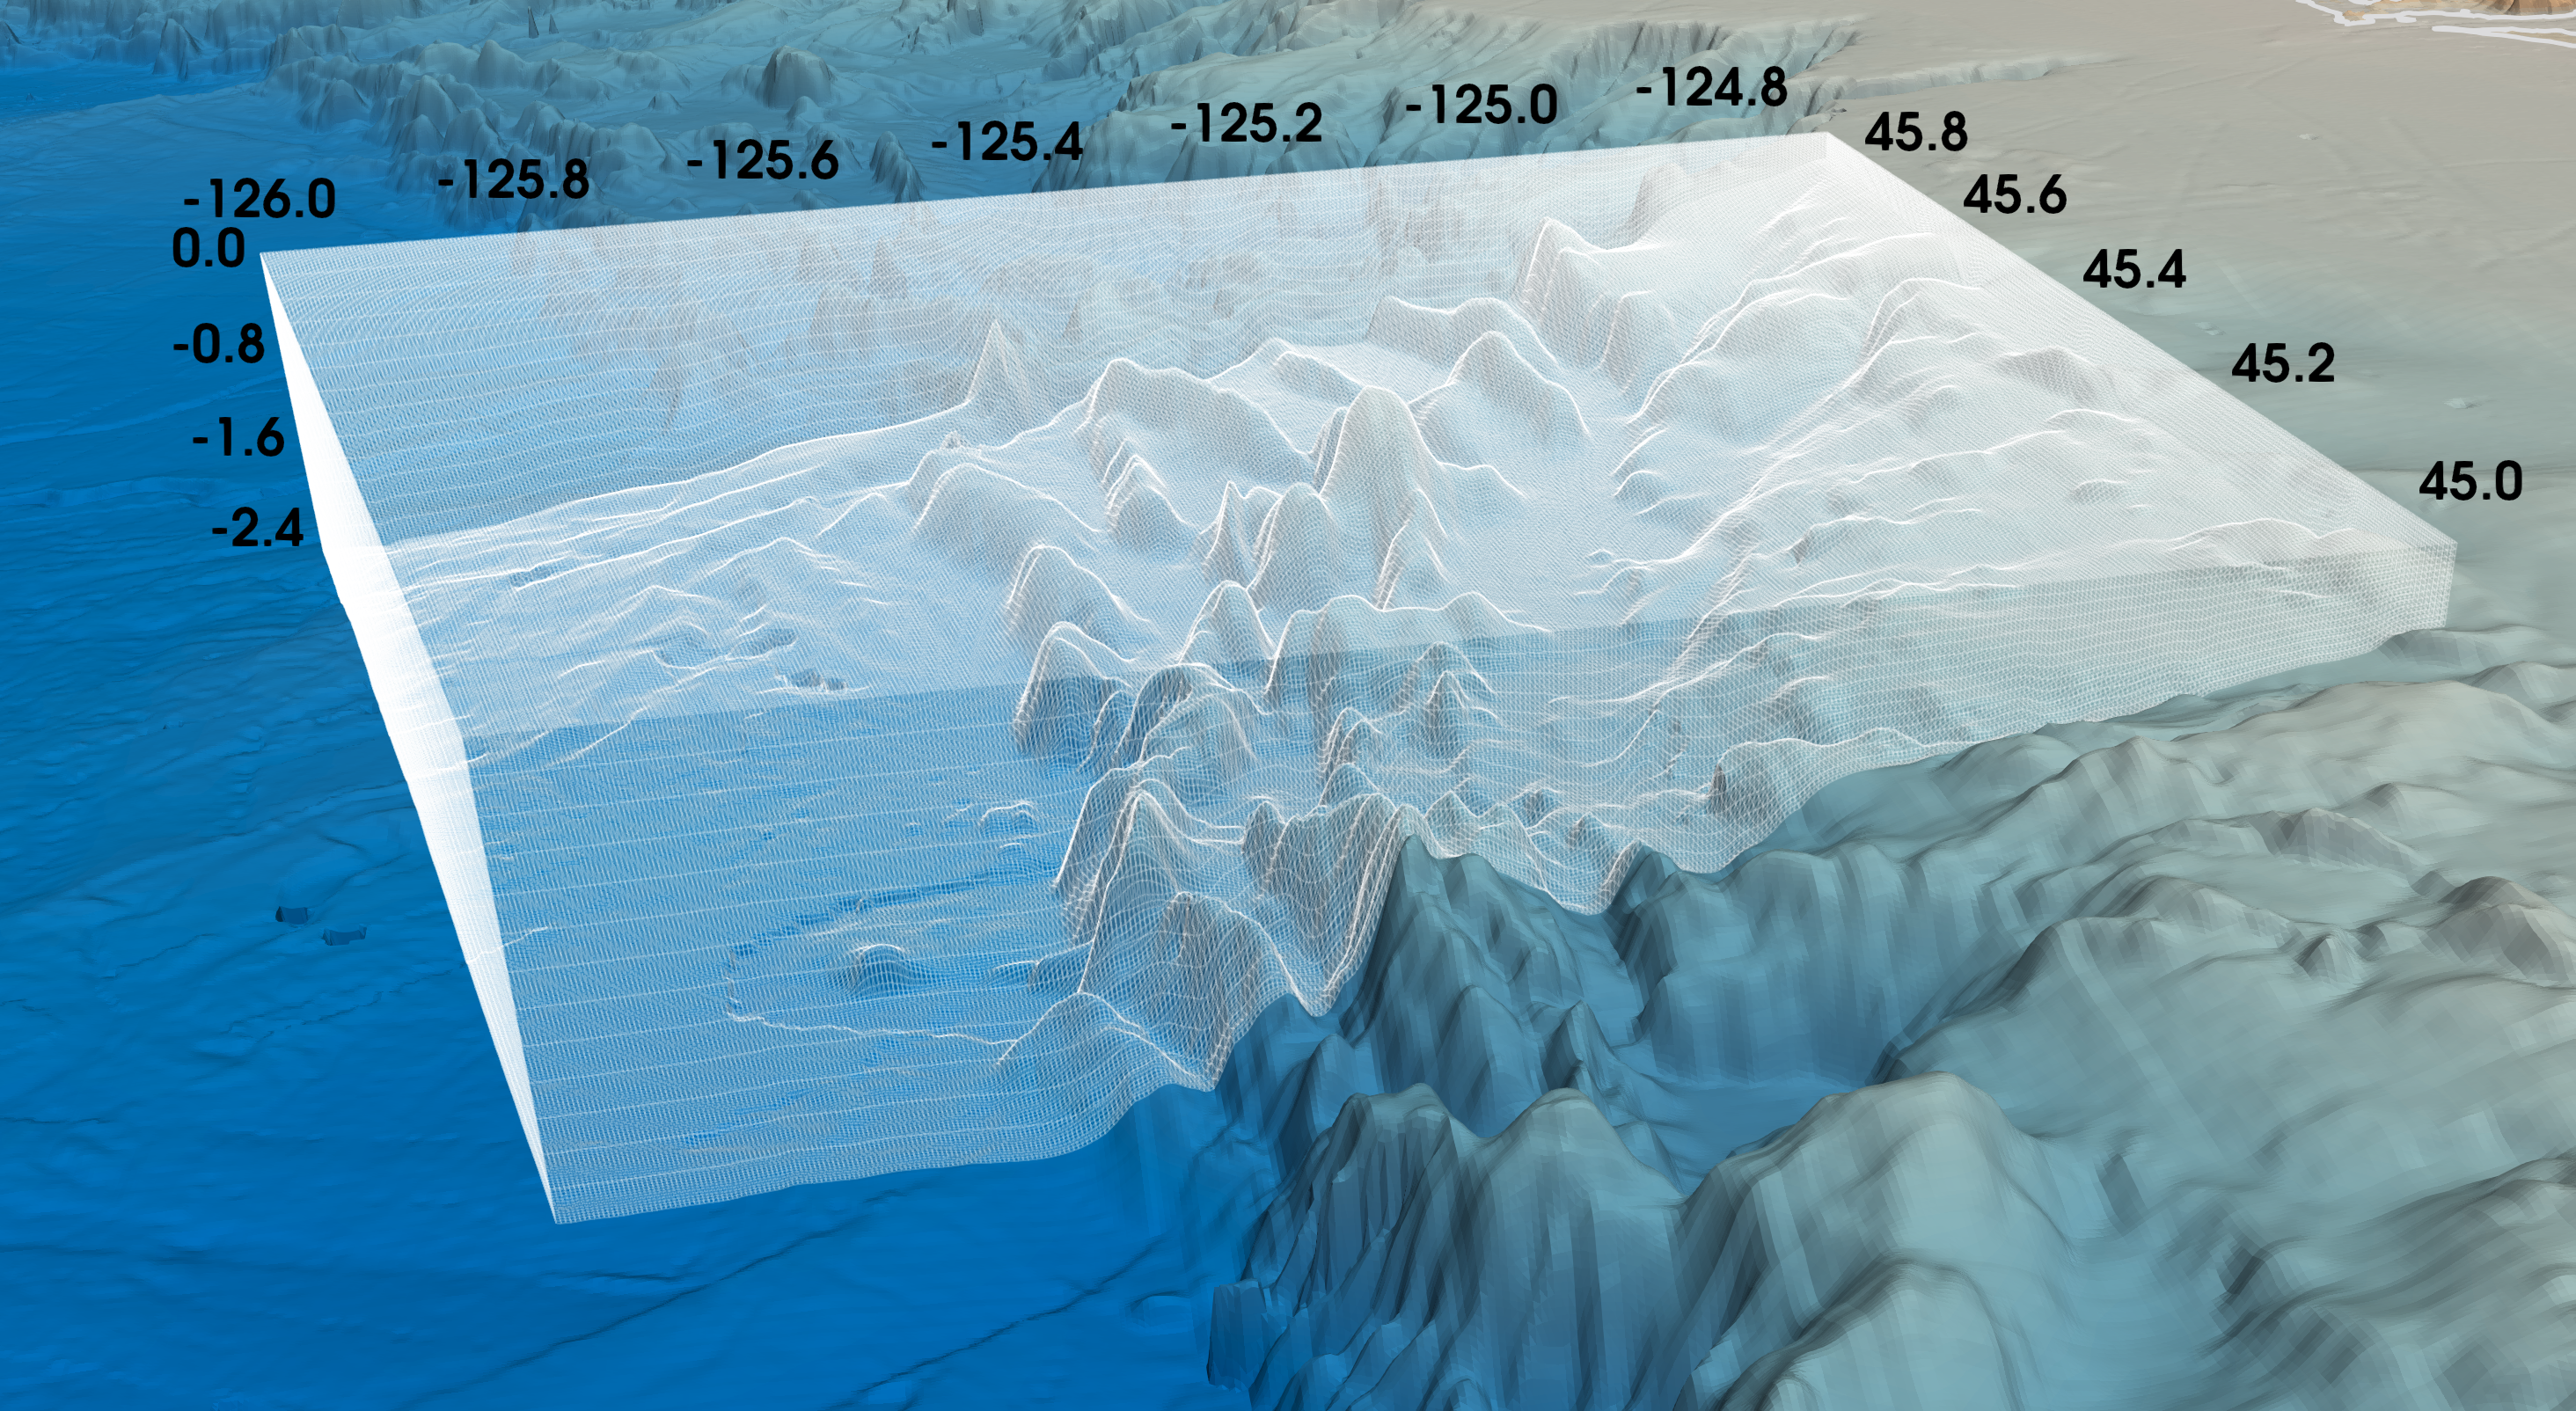
\includegraphics[width=0.95\textwidth]{JMM/images/meshes/CSZ-lat-lon-mesh-2.png}
        \caption{3D hexahedral mesh of a quadrilateral patch of the CSZ in lat. lon. coordinates with ~250m grid spacing}
    \end{figure}
    \begin{itemize}
        \item Vertical scale is exaggerated
    \end{itemize}
\end{frame}